\chapter{Proposed Methodology}
\label{Proposed_Methodology}

This chapter presents the comprehensive methodology for the LD2450 mmWave Indoor Positioning System, detailing the three-phase architectural evolution, hardware configuration, continuous UART data parsing protocols, and network synchronization mechanisms. The proposed solution emphasizes a systematic progression from single-node boundary validation to multi-node spatial coverage, culminating in a fully aggregated, real-time centralized tracking matrix.

\section{System Architectural Phases}
\label{sec:system-phases}

The IPS employs a phased architectural approach that ensures incremental complexity management. Each phase builds upon the previous one while maintaining the core ESP32 parsing algorithms and data structures.

\subsection{Phase 1: Single-Node Boundary Validation}
\label{subsec:phase1}

Phase 1 establishes the foundational data ingestion and environmental modeling framework. In this configuration, a single LD2450 mmWave sensor is deployed facing a controlled perimeter. The sensor actively transmits FMCW chirps and natively computes the Cartesian (X, Y) coordinates of any dynamic target traversing its field of view. 

The communication flow is strictly unidirectional: the LD2450 outputs a continuous hexadecimal UART byte stream to its host ESP32 microcontroller. The ESP32 parses these frames, extracts the target IDs, coordinates, and velocity metrics, and forwards this data over a local Wi-Fi connection to a PC for logging.

This phase serves multiple critical purposes:
\begin{itemize}
    \item \textbf{Buffer Stability:} Tuning the ESP32's asynchronous serial buffer to parse the 256,000 bps UART stream without dropping frames.
    \item \textbf{Digital Bounding:} Establishing mathematically strict X and Y coordinate limits within the ESP32 code to filter out phantom reflections bouncing off exterior walls.
    \item \textbf{Baseline Ground Truth:} Comparing the LD2450's reported coordinates against measured, physical ground-truth markers on the floor.
\end{itemize}

The static positioning of the radar node ensures high reproducibility of results. Expected positioning precision in this phase is $\pm$5-10 cm within the established visual field.

\subsection{Phase 2: Multi-Node Spatial Coverage}
\label{subsec:phase2}

Phase 2 extends the system to support a massive spatial footprint by resolving the line-of-sight occlusion vulnerability intrinsic to mmWave technology. This approach addresses the fundamental challenge of "shadowing," where a target becomes invisible to the radar because they stepped behind a dense pillar or another human.

The Multi-Node architecture deploys multiple LD2450 and ESP32 pairs (sensor clusters) positioned at perpendicular or opposing angles within the same room. Rather than communicating with each other, they operate to overlap their geometrical fields of view:
\begin{itemize}
    \item \textbf{Node A} monitors the East-to-West traversal axis.
    \item \textbf{Node B} monitors the North-to-South traversal axis.
    \item Both nodes independently parse their UART radars.
\end{itemize}

Key advantages of this spatial coverage include:
\begin{itemize}
    \item \textbf{Occlusion Resilience:} If Node A's line-of-sight is blocked, Node B seamlessly maintains the coordinate lock.
    \item \textbf{Extended Range:} Linking sensor fields allows tracking across massive commercial floors.
    \item \textbf{Confidence Boosting:} If both nodes detect the same target, the overlapping coordinate vectors serve to mathematically reinforce the accuracy of the reading.
\end{itemize}

\subsection{Phase 3: Central Aggregation and Visualization}
\label{subsec:phase3}

Phase 3 represents the most advanced configuration, transforming disparate node clusters into a fully synchronized positioning ecosystem. In this phase, every ESP32 node continuously packages its parsed mmWave data and transmits it wirelessly to a Central Gateway.

The Gateway aggregates these overlapping measurements and applies backend processing:
\begin{itemize}
    \item \textbf{Coordinate Transformation:} Translating the relative local (X, Y) coordinates of each sensor node into a global room map.
    \item \textbf{Deduplication Algorithm:} Recognizing when two sensors are tracking the same individual and fusing those two datasets into a single, highly confident trajectory point.
    \item \textbf{Real-Time Rendering:} Streaming the finalized geometrical matrix to a web-based dashboard or external application.
\end{itemize}

\subsection{Phase Compatibility and Evolution}
\label{subsec:phase-compatibility}

A critical design principle is maintaining backwards compatibility across all three phases. The same UART ingestion loops, framing logic, and standardized data structures are used throughout. Nodes can scale from isolated testing environments to networked commercial systems purely through software scaling.

Figure~\ref{fig:system-architecture} illustrates the three-phase architectural evolution and the communication patterns in each configuration.

\section{Hardware Setup and System Layout}
\label{sec:hardware-setup}

The IPS testbed employs commercially available components configured in a controlled indoor environment to ensure measurement reproducibility.

\subsection{Component Specification}
\label{subsec:components}

The system comprises the following hardware components:

\begin{itemize}
    \item \textbf{ESP32 Microcontrollers:} Development boards serving as host processors and network transceivers. Each board features a dual-core processor uniquely suited to dedicating one core entirely to UART Serial parsing, and the second core to Wi-Fi/ESP-NOW communication.
    
    \item \textbf{LD2450 mmWave Radar:} High-frequency 24GHz radar modules. They connect to the ESP32 via standard TX and RX pins. No external analog-to-digital converters are required since the module features internal DSP.
    
    \item \textbf{Power Supply:} Individual 5V power banks for each Node to eliminate ground loop AC interference and facilitate completely untethered wall-mounting.
    
    \item \textbf{Testbed Layout:} A physical floor space measuring roughly 5×5 meters, pre-marked with grid intersections using measuring tape, enabling manual comparison against the radar's digital output.
\end{itemize}

\subsection{Testbed Layout and Coordinate System}
\label{subsec:testbed-layout}

The testbed employs a Cartesian coordinate system with the origin situated exactly at the primary LD2450 sensor's face. 

The sensor placement leverages the physical geometry of the module:
\begin{itemize}
    \item \textbf{X-Axis:} Measures the lateral displacement (left and right of the sensor face).
    \item \textbf{Y-Axis:} Measures the radial distance (directly forward from the sensor).
\end{itemize}

In multi-node Phase 2 setups, secondary sensors require a spatial offset calculation in the central gateway to correctly transpose their localized (X, Y) relative coordinates into the absolute global grid.

Figure~\ref{fig:hardware-layout} illustrates the complete testbed configuration with anchor positions, coordinate system, and sample target placements.

\subsection{Antenna Height and Environmental Considerations}
\label{subsec:antenna-height}

The LD2450 sensors are mounted typically at chest height (approximately 1.2 to 1.5 meters above the floor), angled slightly downwards.
\begin{itemize}
    \item \textbf{Optimal Human Reflection:} Chest-height placement guarantees the radar waves strike the densest mass of the human torso.
    \item \textbf{Ground Reflection Mitigation:} Angling prevents multipath bouncing off polished floors.
\end{itemize}

\subsection{Node Role Assignment}
\label{subsec:node-roles}

Each hardware cluster is assigned a specific role through software configuration:

\begin{itemize}
    \item \textbf{Sensor Nodes:} The ESP32 + LD2450 pairs mounted on the walls. They actively parse the radar, filter boundaries, and transmit JSON-formatted data.
    \item \textbf{Gateway Node:} A central PC or a highly powerful microcomputer (like a Raspberry Pi) operating an MQTT broker or ESP-NOW receiver. It aggregates the networks streams.
\end{itemize}

\section{Data Communication Flow}
\label{sec:data-communication}

The system employs a high-speed telemetric pipeline spanning from raw electromagnetic waves to network-level packets.

\subsection{UART parsing Protocol}
\label{subsec:espnow-protocol}

The fundamental bottleneck resolved in Phase 1 is the UART protocol. The LD2450 transmits data at 256000 bps. The ESP32 utilizes a specialized \texttt{HardwareSerial} library paired with a 256-byte circular buffer to continuously ingest this without blocking the main program execution.

\subsection{Communication Sequence in Phase 1}
\label{subsec:comm-sequence-phase1}

The sequence follows:
\begin{enumerate}
    \item \textbf{Target Movement:} A human target moves. The FMCW chirps reflect back to the LD2450.
    \item \textbf{DSP Execution:} The LD2450 internally calculates the ToF and AoA, deriving precise Cartesian targets.
    \item \textbf{Serial Output:} The LD2450 packages the target IDs, X, and Y values into standard hexadecimal frames starting with header bytes \texttt{0xAA 0xFF} and sends them via UART.
    \item \textbf{Microcontroller Ingestion:} The ESP32 scans the serial buffer looking for the specific header bytes. Upon finding them, it reads the exact next block of frame bytes.
    \item \textbf{Coordinate Bounding:} The ESP32 checks if the extracted X and Y parameters fall inside the programmed room dimensions. If they do not, the packet is instantly discarded as a ghost reflection.
    \item \textbf{Network Transmission:} Validated coordinate structs are transmitted to the Gateway.
\end{enumerate}

Figure~\ref{fig:data-communication-flow} illustrates the complete communication sequence with timing relationships and data structures at each stage.

\subsection{Broadcast Interval and Sampling Strategy}
\label{subsec:broadcast-interval}

The LD2450 updates coordinate arrays several times per second. By pushing data only when a coordinate visibly changes by more than 5cm, we significantly reduce wireless network congestion.

\subsection{Error Handling and Reliability Mechanisms}
\label{subsec:error-handling}

\begin{itemize}
    \item \textbf{Frame Misalignment Detection:} If the footer bytes \texttt{0x55 0xCC} are not found exactly where expected, the frame is corrupted. The ESP32 clears the buffer and waits for the next header.
    \item \textbf{Timeout Triggers:} If the sensor stops detecting a historically tracked target for more than 500ms, the ESP32 automatically transmits a null-status packet indicating that the target has exited the perimeter.
\end{itemize}

\section{Data Packet Structures}
\label{sec:packet-structures}

The ESP32 firmware utilizes specific C-language \texttt{structs} to cast the raw bytes received from the radar into actionable human-readable decimal integers.

\subsection{Target Coordinate Struct}
\label{subsec:target-packet}

The ESP32 breaks down the data frame for a single tracked human into the following structure:

\begin{verbatim}
typedef struct {
    uint8_t target_id;      // Unique radar identifier (0-2)
    int16_t x_pos;          // Lateral distance in mm
    int16_t y_pos;          // Radial distance in mm
    uint16_t velocity;      // Movement speed in cm/s
    uint16_t resolution;    // Sensor confidence metric
} target_data_t;
\end{verbatim}

\textbf{Field Descriptions:}
\begin{itemize}
    \item \textbf{target\_id:} The LD2450 assigns persistent IDs sequentially as targets enter the zone.
    \item \textbf{x\_pos \& y\_pos:} These 16-bit signed integers contain the exact physical distance natively computed by the DSP.
    \item \textbf{velocity:} Facilitates predictive smoothing algorithms on the backend.
\end{itemize}

\subsection{Network Telemetry Packet}
\label{subsec:anchor-packet}

For Phase 2 multi-node operation, the ESP32 attaches its own ID before broadcasting the data:

\begin{verbatim}
typedef struct {
    uint8_t sensor_node;    // ESP32 Node identifier (e.g., Node 1)
    uint32_t timestamp;     // System up-time
    target_data_t targets[3]; // Array holding up to 3 tracked bodies
} network_packet_t;
\end{verbatim}

\subsection{Dataset Format}
\label{subsec:dataset-format}

The Gateway software aggregates these network packets and outputs them as a persistent CSV file utilized for precision analysis:

\begin{table}[H]
\centering
\caption{Dataset Format Structure (Single Node)}
\label{tab:dataset-format}
\begin{tabular}{|c|c|c|c|c|}
\hline
\textbf{Timestamp} & \textbf{Node ID} & \textbf{Target ID} & \textbf{X (mm)} & \textbf{Y (mm)} \\
\hline
10234 & 1 & 0 & -240 & 1500 \\
10280 & 1 & 0 & -220 & 1515 \\
10310 & 1 & 0 & -195 & 1540 \\
\hline
\end{tabular}
\end{table}

\subsection{Extended Dataset Format for Multi-Target}
\label{subsec:extended-dataset}

In crowded environments, the radar fully populates the array, tracking distinct entities concurrently:

\begin{table}[H]
\centering
\caption{Extended Dataset Format for Multi-Target Scenarios}
\label{tab:extended-dataset-format}
\begin{tabular}{|c|c|c|c|c|c|c|}
\hline
\textbf{Timestamp} & \textbf{Tgt0\_X} & \textbf{Tgt0\_Y} & \textbf{Tgt1\_X} & \textbf{Tgt1\_Y} & \textbf{Tgt2\_X} & \textbf{Tgt2\_Y} \\
\hline
14002 & -500 & 1200 & 850 & 2000 & 0 & 0 \\
14050 & -510 & 1220 & 800 & 2010 & 0 & 0 \\
\hline
\end{tabular}
\end{table}

\section{Synchronization and Collision Management}
\label{sec:synchronization}

As the network scales, the central gateway faces thousands of network packets per second. Efficient congestion and collision management algorithms must be implemented.

\subsection{Wireless Conflict Protocols}
\label{subsec:time-slot-protocol}

Unlike RSSI setups which experienced catastrophic interference when two transmitters overlapped, sending mapped telemetry data packets is extremely resilient. The network relies strictly on standard Wi-Fi (CSMA/CA) Carrier-Sense Multiple Access collision avoidance or ESP-NOW sequential acknowledgement. 

\subsubsection{ESP-NOW Interval Control}
\label{subsubsec:time-slot-allocation}

Nodes are programmed to accumulate UART coordinates over a 50ms window before transmitting a singular bulk mesh packet. This drastically reduces overall wireless congestion, guaranteeing that transmission intervals do not overwhelm the aggregator.

\subsection{Data Deduplication (Sensor Fusion)}
\label{subsec:unique-node-id}

The true collision challenge shifts from the wireless spectrum to the Data Layer. If Node A and Node B both see the exact same person, the Gateway receives two disparate coordinate vectors representing a single human.

\subsubsection{Threshold Matching}
\label{subsubsec:interval-control}

The Gateway algorithm employs Euclidean distance thresholds. If Node A reports a target at (Global X=50, Y=100) and Node B reports a target at (Global X=48, Y=105), the algorithm determines the proximity delta is under 15cm. It mathematically fuses these two entries into a single definitive coordinate point, thereby eliminating "ghost tracking clones" created by overlapping sensor fields.

\subsection{Frame Buffer Checksum Alignment}
\label{subsec:mesh-synchronization}

Because serial UART relies purely on timed intervals rather than a separate clock wire, buffer misalignment is highly probable. The ESP32 continuously runs a cyclic redundancy or header-check algorithm against every parsed frame. If the frame deviates by even a solitary byte, the entire batch is wiped. This guarantees that absolutely no corrupted coordinate geometry ever enters the network pipeline.

\section{System Diagrams and Visual Representations}
\label{sec:system-diagrams}

This section presents comprehensive visual representations of the ESP32 IPS architecture, data flows, and operational processes. These diagrams provide intuitive understanding of system components, their interactions, and the evolution across the operational phases.

\subsection{System Architecture Diagram}
\label{subsec:system-architecture-diagram}

Figure~\ref{fig:system-architecture} illustrates the architectural evolution of the system.

\begin{figure}[htbp]
    \centering
    \resizebox{0.95\textwidth}{!}{\begin{tikzpicture}[
    node distance=1.5cm and 2cm,
    box/.style={rectangle, draw, thick, minimum width=2cm, minimum height=0.8cm, align=center, font=\small},
    phase/.style={rectangle, draw, dashed, thick, inner sep=0.5cm},
    arrow/.style={->, thick},
    bidir/.style={<->, thick}
]

% Phase 1: Hands-Free (Single Target)
\node[phase, label={[font=\bfseries]above:Phase 1: Hands-Free (Single Target)}] (phase1) at (0,0) {
    \begin{tikzpicture}[node distance=1cm and 1.5cm, box/.style={rectangle, draw, thick, minimum width=2cm, minimum height=0.8cm, align=center, font=\small}, arrow/.style={->, thick}]
        \node[box, fill=blue!20] (t1) {Target\\Node};
        \node[box, fill=green!20, below left=of t1] (a1) {Anchor 1};
        \node[box, fill=green!20, below=of a1] (a2) {Anchor 2};
        \node[box, fill=green!20, below right=of t1] (a3) {Anchor 3};
        \node[box, fill=green!20, below=of a3] (a4) {Anchor 4};
        \node[box, fill=orange!20, below=2.5cm of t1] (gw1) {Gateway};
        \node[box, fill=red!20, below=of gw1] (pc1) {PC/Logger};
        
        \draw[arrow] (t1) -- node[left, font=\tiny] {Broadcast} (a1);
        \draw[arrow] (t1) -- node[right, font=\tiny] {Broadcast} (a3);
        \draw[arrow] (t1) -- (a2);
        \draw[arrow] (t1) -- (a4);
        \draw[arrow] (a1) -- node[left, font=\tiny] {RSSI} (gw1);
        \draw[arrow] (a2) -- (gw1);
        \draw[arrow] (a3) -- node[right, font=\tiny] {RSSI} (gw1);
        \draw[arrow] (a4) -- (gw1);
        \draw[arrow] (gw1) -- node[right, font=\tiny] {Data} (pc1);
    \end{tikzpicture}
};

% Phase 2: Multi-Target Sequential
\node[phase, label={[font=\bfseries]above:Phase 2: Multi-Target Sequential}, right=4cm of phase1] (phase2) {
    \begin{tikzpicture}[node distance=1.2cm and 1.5cm, box/.style={rectangle, draw, thick, minimum width=2cm, minimum height=0.8cm, align=center, font=\small}, arrow/.style={->, thick}]
        \node[box, fill=blue!20] (t2a) {Target A\\Slot 0-100ms};
        \node[box, fill=blue!20, below=0.4cm of t2a] (t2b) {Target B\\Slot 100-200ms};
        \node[box, fill=blue!20, below=0.4cm of t2b] (t2c) {Target C\\Slot 200-300ms};
        \node[box, fill=green!20, below=2.2cm of t2b] (an) {Anchors\\(All)};
        \node[box, fill=orange!20, below=1.2cm of an] (gw2) {Gateway};
        \node[box, fill=red!20, below=1.2cm of gw2] (pc2) {PC/Logger};
        
        % Curved arrows to avoid overlap
        \draw[arrow] (t2a.south) to[out=-90, in=150] (an.north west);
        \draw[arrow] (t2b.south) -- (an.north);
        \draw[arrow] (t2c.south) to[out=-90, in=30] (an.north east);
        \draw[arrow] (an) -- node[right, font=\tiny, align=center] {Tagged\\RSSI} (gw2);
        \draw[arrow] (gw2) -- node[right, font=\tiny, align=center] {Multi-Target\\Data} (pc2);
    \end{tikzpicture}
};

% Phase 3: All-Nodes Mesh
\node[phase, label={[font=\bfseries]above:Phase 3: All-Nodes Mesh}, right=4cm of phase2] (phase3) {
    \begin{tikzpicture}[node distance=2cm and 2cm]
        \node[box, fill=purple!20] (n1) {Node 1};
        \node[box, fill=purple!20, right=of n1] (n2) {Node 2};
        \node[box, fill=purple!20, below=of n1] (n4) {Node 4};
        \node[box, fill=purple!20, below=of n2] (n3) {Node 3};
        \node[box, fill=orange!20, below=1.5cm of n4] (gw3) {Gateway};
        
        \draw[bidir] (n1) -- node[above, font=\tiny] {RSSI} (n2);
        \draw[bidir] (n2) -- node[right, font=\tiny] {RSSI} (n3);
        \draw[bidir] (n3) -- node[below, font=\tiny] {RSSI} (n4);
        \draw[bidir] (n4) -- node[left, font=\tiny] {RSSI} (n1);
        \draw[bidir] (n1) -- (n3);
        \draw[bidir] (n2) -- (n4);
        
        \draw[arrow] (n1) -- (gw3);
        \draw[arrow] (n2) -- (gw3);
        \draw[arrow] (n3) -- (gw3);
        \draw[arrow] (n4) -- (gw3);
    \end{tikzpicture}
};

% Evolution arrows
\draw[->, ultra thick, blue] ([xshift=0.5cm]phase1.east) -- ([xshift=-0.5cm]phase2.west) node[midway, above] {Evolution};
\draw[->, ultra thick, blue] ([xshift=0.5cm]phase2.east) -- ([xshift=-0.5cm]phase3.west) node[midway, above] {Evolution};

\end{tikzpicture}
}
    \caption{Three-Phase System Architecture Evolution showing communication patterns and node roles in each operational mode}
    \label{fig:system-architecture}
\end{figure}

\subsection{Data Communication Flow Diagram}
\label{subsec:data-flow-diagram}

Figure~\ref{fig:data-communication-flow} presents a detailed sequence diagram showing the temporal flow of data through the system.

\begin{figure}[htbp]
    \centering
    \resizebox{0.9\textwidth}{!}{\begin{tikzpicture}[
    node distance=1.5cm,
    actor/.style={rectangle, draw, thick, minimum width=2cm, minimum height=0.8cm, align=center, font=\small},
    message/.style={->, thick},
    note/.style={rectangle, draw, dashed, fill=yellow!20, font=\tiny, align=left}
]

% Actors
\node[actor, fill=blue!20] (target) {Target\\Node};
\node[actor, fill=green!20, right=of target] (a1) {Anchor 1};
\node[actor, fill=green!20, right=of a1] (a2) {Anchor 2};
\node[actor, fill=green!20, right=of a2] (a3) {Anchor 3};
\node[actor, fill=green!20, right=of a3] (a4) {Anchor 4};
\node[actor, fill=orange!20, right=of a4] (gw) {Gateway};
\node[actor, fill=red!20, right=of gw] (pc) {PC/\\Logger};

% Lifelines
\draw[dashed] (target) -- ++(0,-12);
\draw[dashed] (a1) -- ++(0,-12);
\draw[dashed] (a2) -- ++(0,-12);
\draw[dashed] (a3) -- ++(0,-12);
\draw[dashed] (a4) -- ++(0,-12);
\draw[dashed] (gw) -- ++(0,-12);
\draw[dashed] (pc) -- ++(0,-12);

% Broadcast messages
\draw[message] ([yshift=-1cm]target.south) -- node[above, font=\tiny, sloped] {ESP-NOW Broadcast} ([yshift=-1cm]a1.south);
\draw[message] ([yshift=-1.5cm]target.south) -- node[above, font=\tiny, sloped] {ESP-NOW Broadcast} ([yshift=-1.5cm]a2.south);
\draw[message] ([yshift=-2cm]target.south) -- node[above, font=\tiny, sloped] {ESP-NOW Broadcast} ([yshift=-2cm]a3.south);
\draw[message] ([yshift=-2.5cm]target.south) -- node[above, font=\tiny, sloped] {ESP-NOW Broadcast} ([yshift=-2.5cm]a4.south);

% Note about packet structure
\node[note, below=3cm of target] (note1) {
    target\_packet\_t:\\
    - target\_id\\
    - timestamp\\
    - message
};

% Note about RSSI recording
\node[note, below=4cm of a2] (note2) {
    Record RSSI\\
    \& Timestamp
};

% Anchor to Gateway messages
\draw[message] ([yshift=-5.5cm]a1.south) -- node[above, font=\tiny, sloped] {anchor\_data\_t} ([yshift=-5.5cm]gw.south);
\draw[message] ([yshift=-6cm]a2.south) -- node[above, font=\tiny, sloped] {anchor\_data\_t} ([yshift=-6cm]gw.south);
\draw[message] ([yshift=-6.5cm]a3.south) -- node[above, font=\tiny, sloped] {anchor\_data\_t} ([yshift=-6.5cm]gw.south);
\draw[message] ([yshift=-7cm]a4.south) -- node[above, font=\tiny, sloped] {anchor\_data\_t} ([yshift=-7cm]gw.south);

% Note about anchor data structure
\node[note, below=8cm of a3] (note3) {
    anchor\_data\_t:\\
    - anchor\_id\\
    - rssi\\
    - timestamp
};

% Gateway to PC message
\draw[message] ([yshift=-9.5cm]gw.south) -- node[above, font=\tiny] {Aggregated Dataset} ([yshift=-9.5cm]pc.south);

% Note about dataset format
\node[note, below=10.5cm of gw] (note4) {
    Dataset Format:\\
    X, Y, RSSI\_A1,\\
    RSSI\_A2, RSSI\_A3,\\
    RSSI\_A4
};

\end{tikzpicture}
}
    \caption{Data Communication Flow Sequence showing packet transmission and processing processes}
    \label{fig:data-communication-flow}
\end{figure}

\subsection{Hardware Layout Diagram}
\label{subsec:hardware-layout-diagram}

Figure~\ref{fig:hardware-layout} depicts the physical testbed configuration.

\begin{figure}[htbp]
    \centering
    \resizebox{0.85\textwidth}{!}{\begin{tikzpicture}[
    scale=0.12,
    anchor/.style={circle, draw, thick, fill=green!30, minimum size=1cm, font=\bfseries},
    target/.style={circle, draw, thick, fill=blue!30, minimum size=0.8cm, font=\small},
    dimension/.style={<->, thick, >=stealth}
]

% Draw grid
\draw[step=10, gray, very thin] (0,0) grid (70,50);
\draw[step=10, gray, thick] (0,0) grid (70,50);

% Draw border
\draw[very thick] (0,0) rectangle (70,50);

% Place anchors at corners - Labels with coordinates only
\node[anchor, label={below left:\textbf{A1 (0,0)}}] (a1) at (0,0) {};
\node[anchor, label={below right:\textbf{A2 (70,0)}}] (a2) at (70,0) {};
\node[anchor, label={above left:\textbf{A3 (0,50)}}] (a3) at (0,50) {};
\node[anchor, label={above right:\textbf{A4 (70,50)}}] (a4) at (70,50) {};

% Place sample target positions
\node[target, label={above:T1}] (t1) at (20,15) {T};
\node[target, label={above:T2}] (t2) at (35,30) {T};
\node[target, label={above:T3}] (t3) at (50,20) {T};

% Draw signal lines from targets to anchors (dashed)
\draw[dashed, blue!50, thin] (t1) -- (a1);
\draw[dashed, blue!50, thin] (t1) -- (a2);
\draw[dashed, blue!50, thin] (t1) -- (a3);
\draw[dashed, blue!50, thin] (t1) -- (a4);

% Dimensions
\draw[dimension] (0,-5) -- (70,-5) node[midway, below] {70 cm};
\draw[dimension] (-5,0) -- (-5,50) node[midway, left, rotate=90] {50 cm};

% Coordinate system labels
\node[font=\small] at (35,-10) {X-axis (cm)};
\node[font=\small, rotate=90] at (-10,25) {Y-axis (cm)};

% Add coordinate markers
\foreach \x in {0,10,20,30,40,50,60,70} {
    \node[font=\tiny, below] at (\x,-1) {\x};
}
\foreach \y in {0,10,20,30,40,50} {
    \node[font=\tiny, left] at (-1,\y) {\y};
}

% Legend
\node[anchor, minimum size=0.6cm] at (60,-8) {};
\node[font=\small, right] at (61,-8) {Anchor Node};
\node[target, minimum size=0.5cm] at (60,-12) {};
\node[font=\small, right] at (61,-12) {Target Node};

% Title
\node[font=\large\bfseries] at (35,55) {ESP32 IPS Testbed Layout};

% Add note about antenna height
\node[rectangle, draw, dashed, fill=yellow!20, font=\small, align=left] at (35,-18) {
    Note: All antennas at 10 cm height\\
    Grid spacing: 10 cm
};

\end{tikzpicture}
}
    \caption{Physical Testbed Layout showing coordinate system and sample target locations}
    \label{fig:hardware-layout}
\end{figure}

\subsection{Data Flow Diagrams (DFD)}
\label{subsec:dfd-diagrams}

Data Flow Diagrams provide structured representations of data processing and storage within the system.

\subsubsection{DFD Level 0 - Context Diagram}
\label{subsubsec:dfd-level0}

Figure~\ref{fig:dfd-level0} presents the context-level view.

\begin{figure}[htbp]
    \centering
    \resizebox{0.9\textwidth}{!}{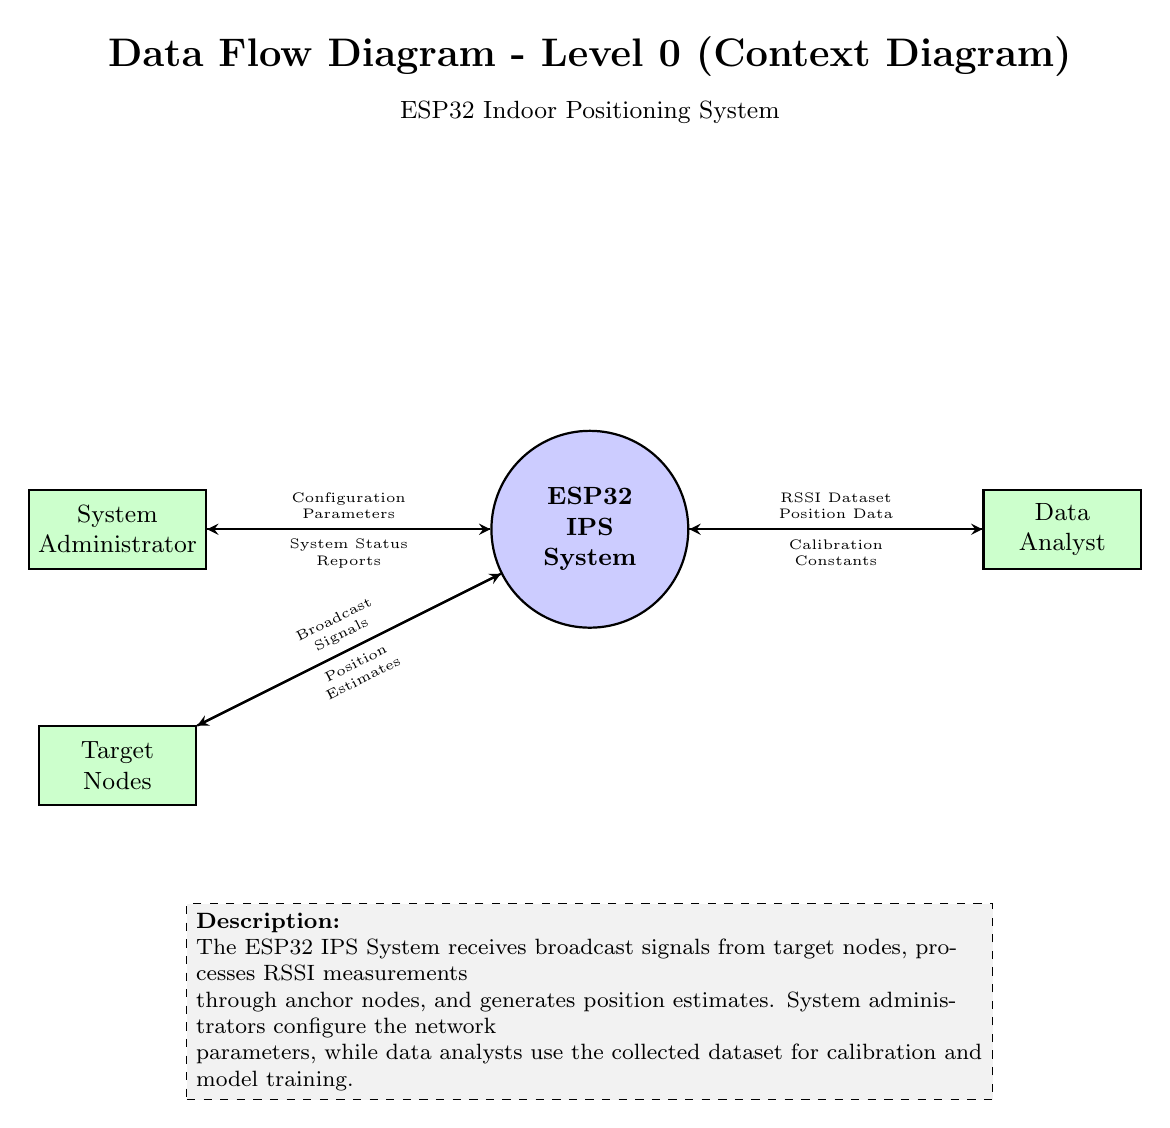
\begin{tikzpicture}[
    node distance=3cm,
    process/.style={circle, draw, thick, minimum size=2.5cm, align=center, font=\small\bfseries, fill=blue!20},
    entity/.style={rectangle, draw, thick, minimum width=2cm, minimum height=1cm, align=center, font=\small, fill=green!20},
    datastore/.style={rectangle, draw, thick, minimum width=2.5cm, minimum height=0.8cm, align=center, font=\small, fill=yellow!20},
    flow/.style={->, thick, >=stealth}
]

% Title
\node[font=\Large\bfseries] at (0,6) {Data Flow Diagram - Level 0 (Context Diagram)};
\node[font=\small] at (0,5.3) {ESP32 Indoor Positioning System};

% External Entities
\node[entity] (user) at (-6,0) {System\\Administrator};
\node[entity] (target) at (-6,-3) {Target\\Nodes};
\node[entity] (analyst) at (6,0) {Data\\Analyst};

% Central Process
\node[process] (system) at (0,0) {ESP32\\IPS\\System};

% Data Flows
\draw[flow] (user) -- node[above, font=\tiny, sloped, align=center] {Configuration\\Parameters} (system);
\draw[flow] (system) -- node[below, font=\tiny, sloped, align=center] {System Status\\Reports} (user);

\draw[flow] (target) -- node[above, font=\tiny, sloped, align=center] {Broadcast\\Signals} (system);
\draw[flow] (system) -- node[below, font=\tiny, sloped, align=center] {Position\\Estimates} (target);

\draw[flow] (system) -- node[above, font=\tiny, sloped, align=center] {RSSI Dataset\\Position Data} (analyst);
\draw[flow] (analyst) -- node[below, font=\tiny, sloped, align=center] {Calibration\\Constants} (system);

% Description box
\node[rectangle, draw, dashed, fill=gray!10, text width=10cm, align=left, font=\footnotesize] at (0,-6) {
    \textbf{Description:}\\
    The ESP32 IPS System receives broadcast signals from target nodes, processes RSSI measurements\\
    through anchor nodes, and generates position estimates. System administrators configure the network\\
    parameters, while data analysts use the collected dataset for calibration and model training.
};

\end{tikzpicture}
}
    \caption{Data Flow Diagram Level 0 (Context Diagram) showing system boundaries and external entity interactions}
    \label{fig:dfd-level0}
\end{figure}

\subsubsection{DFD Level 1 - Detailed Process Decomposition}
\label{subsubsec:dfd-level1}

Figure~\ref{fig:dfd-level1} decomposes the system into detailed processes.

\begin{figure}[htbp]
    \centering
    \resizebox{0.95\textwidth}{!}{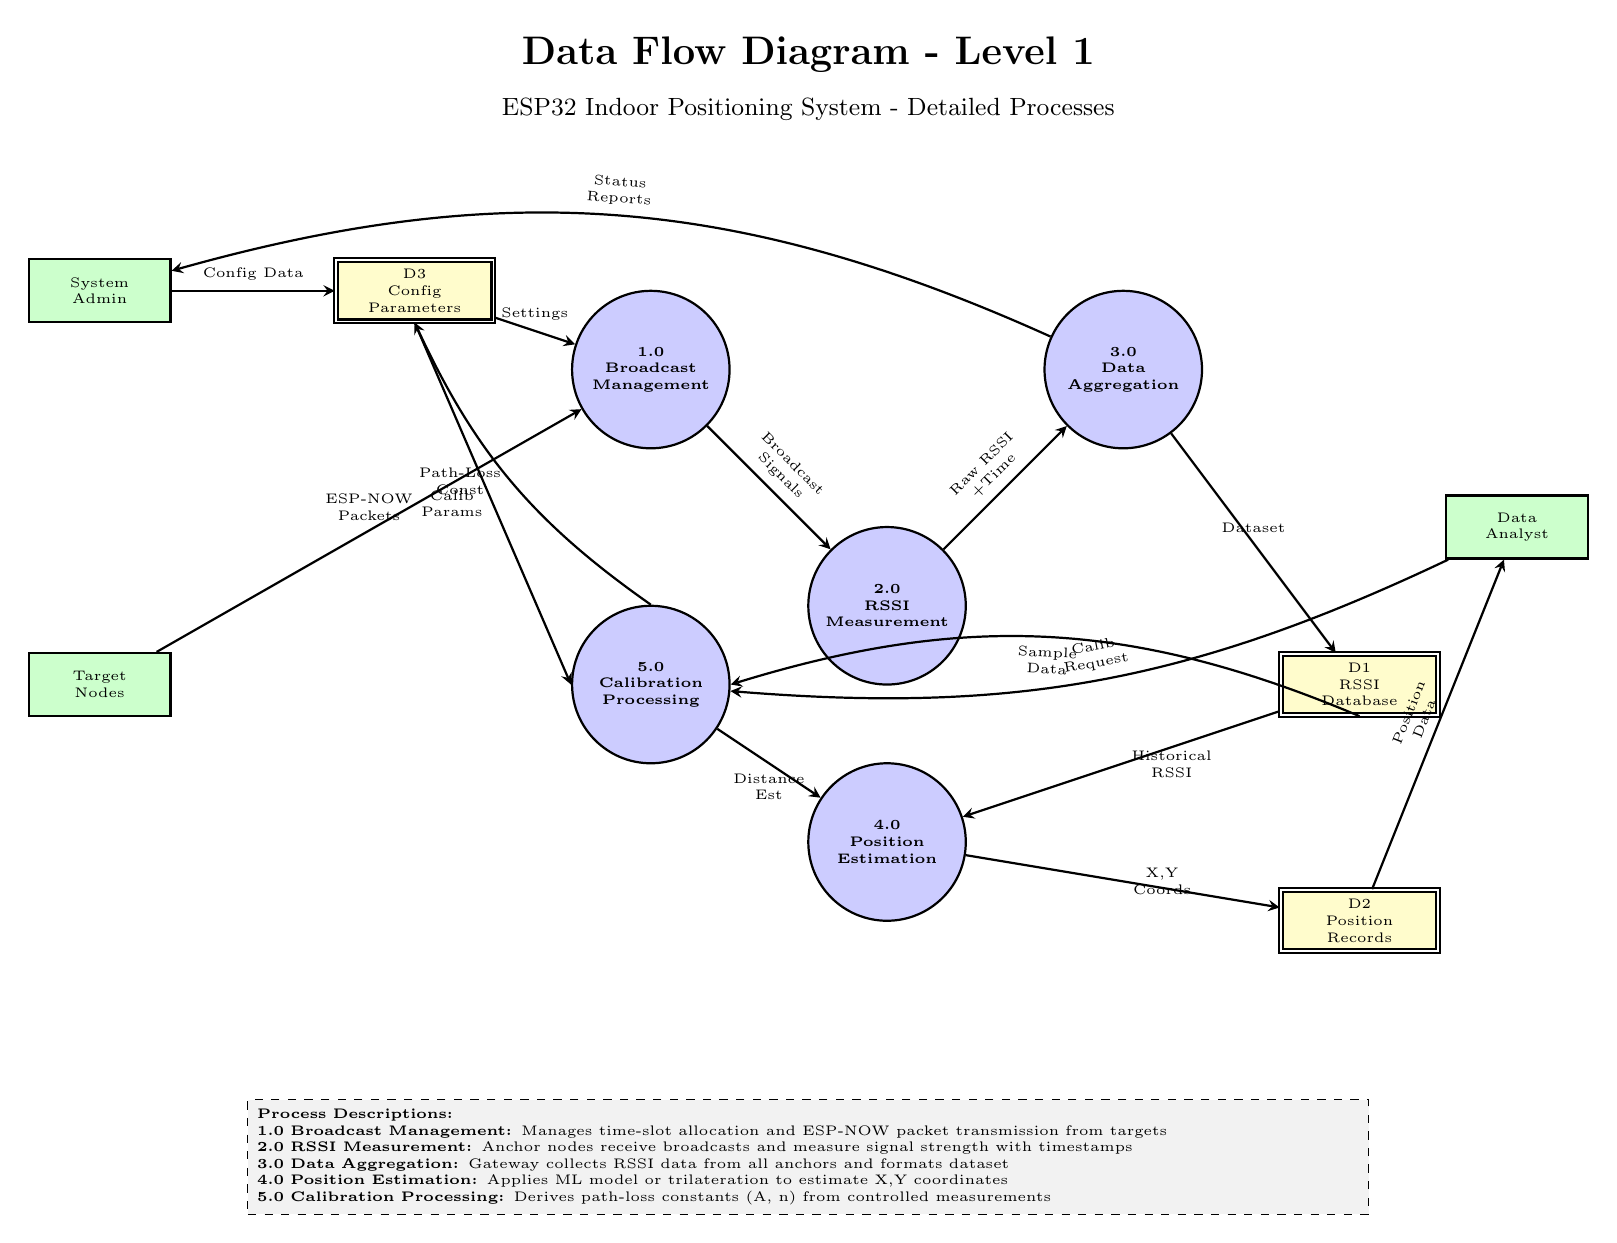
\begin{tikzpicture}[
    node distance=3cm and 4cm,
    process/.style={circle, draw, thick, minimum size=2cm, align=center, font=\tiny\bfseries, fill=blue!20},
    entity/.style={rectangle, draw, thick, minimum width=1.8cm, minimum height=0.8cm, align=center, font=\tiny, fill=green!20},
    datastore/.style={rectangle, draw, thick, minimum width=2cm, minimum height=0.6cm, align=center, font=\tiny, fill=yellow!20, double},
    flow/.style={->, thick, >=stealth},
    label/.style={font=\tiny}
]

% Title
\node[font=\Large\bfseries] at (0,9) {Data Flow Diagram - Level 1};
\node[font=\small] at (0,8.3) {ESP32 Indoor Positioning System - Detailed Processes};

% External Entities - Positioned at edges
\node[entity] (user) at (-9,6) {System\\Admin};
\node[entity] (target) at (-9,1) {Target\\Nodes};
\node[entity] (analyst) at (9,3) {Data\\Analyst};

% Data Stores - Positioned to minimize crossings
\node[datastore] (d3) at (-5,6) {D3\\Config\\Parameters};
\node[datastore] (d1) at (7,1) {D1\\RSSI\\Database};
\node[datastore] (d2) at (7,-2) {D2\\Position\\Records};

% Processes - Arranged in logical flow order
\node[process] (p1) at (-2,5) {1.0\\Broadcast\\Management};
\node[process] (p2) at (1,2) {2.0\\RSSI\\Measurement};
\node[process] (p3) at (4,5) {3.0\\Data\\Aggregation};
\node[process] (p4) at (1,-1) {4.0\\Position\\Estimation};
\node[process] (p5) at (-2,1) {5.0\\Calibration\\Processing};

% Data Flows - User/Admin to Config
\draw[flow] (user) -- node[above, label] {Config Data} (d3);
\draw[flow] (d3) -- node[above, label] {Settings} (p1);
\draw[flow] (d3.south) -- node[left, label, align=center] {Calib\\Params} (p5.west);

% Data Flows - Target to Broadcast
\draw[flow] (target) -- node[above, label, align=center] {ESP-NOW\\Packets} (p1);

% Data Flows - Main processing chain
\draw[flow] (p1) -- node[above, label, sloped, align=center] {Broadcast\\Signals} (p2);
\draw[flow] (p2) -- node[above, label, sloped, align=center] {Raw RSSI\\+Time} (p3);
\draw[flow] (p3) -- node[above, label] {Dataset} (d1);

% Data Flows - RSSI to Position Estimation
\draw[flow] (d1) -- node[right, label, align=center] {Historical\\RSSI} (p4);
\draw[flow] (p4) -- node[right, label, align=center] {X,Y\\Coords} (d2);

% Data Flows - Output to Analyst
\draw[flow] (d2) -- node[above, label, sloped, align=center] {Position\\Data} (analyst);

% Data Flows - Calibration loop
\draw[flow] (analyst) to[bend left=15] node[above, label, sloped, align=center] {Calib\\Request} (p5);
\draw[flow] (d1.south) to[bend right=20] node[below, label, sloped, align=center] {Sample\\Data} (p5.east);
\draw[flow] (p5) -- node[below, label, align=center] {Distance\\Est} (p4);
\draw[flow] (p5.north) to[bend left=15] node[left, label, align=center] {Path-Loss\\Const} (d3.south);

% Data Flows - Status feedback
\draw[flow] (p3) to[bend right=20] node[above, label, sloped, align=center] {Status\\Reports} (user);

% Legend
\node[rectangle, draw, dashed, fill=gray!10, text width=14cm, align=left, font=\tiny] at (0,-5) {
    \textbf{Process Descriptions:}\\
    \textbf{1.0 Broadcast Management:} Manages time-slot allocation and ESP-NOW packet transmission from targets\\
    \textbf{2.0 RSSI Measurement:} Anchor nodes receive broadcasts and measure signal strength with timestamps\\
    \textbf{3.0 Data Aggregation:} Gateway collects RSSI data from all anchors and formats dataset\\
    \textbf{4.0 Position Estimation:} Applies ML model or trilateration to estimate X,Y coordinates\\
    \textbf{5.0 Calibration Processing:} Derives path-loss constants (A, n) from controlled measurements
};

\end{tikzpicture}
}
    \caption{Data Flow Diagram Level 1 showing detailed process decomposition, data stores, and inter-process data flows}
    \label{fig:dfd-level1}
\end{figure}

\subsection{Entity-Relationship Diagram}
\label{subsec:er-diagram}

Figure~\ref{fig:er-diagram} presents the database schema.

\begin{figure}[htbp]
    \centering
    \resizebox{0.95\textwidth}{!}{\begin{tikzpicture}[
    node distance=3cm and 4cm,
    entity/.style={rectangle, draw, thick, minimum width=2.8cm, minimum height=1.3cm, align=center, font=\small\bfseries, fill=blue!20},
    attribute/.style={ellipse, draw, thick, minimum width=1.6cm, minimum height=0.85cm, align=center, font=\tiny, fill=green!20},
    relationship/.style={diamond, draw, thick, minimum width=2.2cm, minimum height=1.3cm, align=center, font=\tiny\bfseries, fill=yellow!20},
    key/.style={underline},
    line/.style={thick}
]

% Title
\node[font=\Large\bfseries] at (0,11) {Entity-Relationship Diagram};
\node[font=\small] at (0,10.3) {ESP32 Indoor Positioning System Database Schema};

% Entities - Increased spacing
\node[entity] (node) at (-7,6) {NODE};
\node[entity] (measurement) at (0,6) {MEASUREMENT};
\node[entity] (position) at (7,6) {POSITION};
\node[entity] (calibration) at (-7,0) {CALIBRATION};
\node[entity] (session) at (7,0) {SESSION};

% Node Attributes - Better positioning
\node[attribute] (node_id) at (-9.5,8.5) {\underline{node\_id}};
\node[attribute] (node_type) at (-7,9) {node\_type};
\node[attribute] (mac_addr) at (-4.5,8.5) {mac\_address};
\node[attribute] (location_x) at (-9.5,6) {location\_x};
\node[attribute] (location_y) at (-9.5,4.5) {location\_y};
\node[attribute] (antenna_h) at (-4.5,4.5) {antenna\_height};

% Measurement Attributes - Spread out more
\node[attribute] (meas_id) at (0,9) {\underline{measurement\_id}};
\node[attribute] (rssi) at (-2.5,8.5) {rssi\_value};
\node[attribute] (timestamp) at (2.5,8.5) {timestamp};
\node[attribute] (packet_id) at (0,3.5) {packet\_id};

% Position Attributes - Better spacing
\node[attribute] (pos_id) at (7,9) {\underline{position\_id}};
\node[attribute] (est_x) at (9.5,8.5) {estimated\_x};
\node[attribute] (est_y) at (9.5,7) {estimated\_y};
\node[attribute] (confidence) at (9.5,5) {confidence};
\node[attribute] (method) at (9.5,3.5) {method};

% Calibration Attributes - More space
\node[attribute] (cal_id) at (-9.5,0) {\underline{calibration\_id}};
\node[attribute] (param_a) at (-7,-1.5) {parameter\_A};
\node[attribute] (param_n) at (-4.5,0) {parameter\_n};
\node[attribute] (cal_date) at (-7,2) {calibration\_date};

% Session Attributes - Better layout
\node[attribute] (sess_id) at (9.5,0) {\underline{session\_id}};
\node[attribute] (start_time) at (7,-1.5) {start\_time};
\node[attribute] (end_time) at (7,2) {end\_time};
\node[attribute] (phase) at (4.5,0) {phase\_type};

% Relationships - Adjusted positions
\node[relationship] (transmits) at (-3.5,6) {TRANS-\\MITS};
\node[relationship] (receives) at (3.5,6) {RECEIVES};
\node[relationship] (generates) at (3.5,3) {GENE-\\RATES};
\node[relationship] (uses) at (-3.5,3) {USES};
\node[relationship] (belongs) at (0,0) {BELONGS\\TO};

% Connections - Node to Transmits (horizontal)
\draw[line] (node.east) -- (transmits.west);
\draw[line] (transmits.east) -- (measurement.west);
\node[font=\tiny] at (-5.5,6.5) {1};
\node[font=\tiny] at (-1.5,6.5) {N};

% Connections - Measurement to Receives (horizontal)
\draw[line] (measurement.east) -- (receives.west);
\draw[line] (receives.east) -- (position.west);
\node[font=\tiny] at (1.5,6.5) {N};
\node[font=\tiny] at (5.5,6.5) {1};

% Connections - Position to Generates (curved to avoid crossing)
\draw[line] (position.south) to[bend right=20] (generates.north);
\draw[line] (generates.west) to[bend right=15] (measurement.south);
\node[font=\tiny] at (6,3.5) {1};
\node[font=\tiny] at (1.5,3.5) {N};

% Connections - Calibration to Uses (curved to avoid crossing)
\draw[line] (calibration.north) to[bend left=20] (uses.south);
\draw[line] (uses.north) to[bend left=15] (node.south);
\node[font=\tiny] at (-6,3.5) {N};
\node[font=\tiny] at (-6,4.5) {1};

% Connections - Session to Belongs (curved)
\draw[line] (session.north) to[bend right=20] (belongs.south);
\draw[line] (belongs.north) to[bend right=15] (measurement.south);
\node[font=\tiny] at (5,0.5) {1};
\node[font=\tiny] at (1.5,0.5) {N};

% Attribute Connections - Node
\draw[line] (node_id) -- (node.north west);
\draw[line] (node_type) -- (node.north);
\draw[line] (mac_addr) -- (node.north east);
\draw[line] (location_x) -- (node.west);
\draw[line] (location_y) -- (node.south west);
\draw[line] (antenna_h) -- (node.south east);

% Attribute Connections - Measurement
\draw[line] (meas_id) -- (measurement.north);
\draw[line] (rssi) -- (measurement.north west);
\draw[line] (timestamp) -- (measurement.north east);
\draw[line] (packet_id) -- (measurement.south);

% Attribute Connections - Position
\draw[line] (pos_id) -- (position.north);
\draw[line] (est_x) -- (position.north east);
\draw[line] (est_y) -- (position.east);
\draw[line] (confidence) -- (position.east);
\draw[line] (method) -- (position.south east);

% Attribute Connections - Calibration
\draw[line] (cal_id) -- (calibration.west);
\draw[line] (param_a) -- (calibration.south);
\draw[line] (param_n) -- (calibration.east);
\draw[line] (cal_date) -- (calibration.north);

% Attribute Connections - Session
\draw[line] (sess_id) -- (session.east);
\draw[line] (start_time) -- (session.south);
\draw[line] (end_time) -- (session.north);
\draw[line] (phase) -- (session.west);

% Legend - Moved further down to avoid overlap
\node[rectangle, draw, dashed, fill=gray!10, text width=14cm, align=left, font=\tiny] at (0,-4.5) {
    \textbf{Entity Descriptions:}\\
    \textbf{NODE:} Represents ESP32 devices (targets, anchors, gateway) with unique IDs and physical locations\\
    \textbf{MEASUREMENT:} Stores individual RSSI measurements with timestamps from anchor nodes\\
    \textbf{POSITION:} Contains estimated X,Y coordinates derived from RSSI measurements\\
    \textbf{CALIBRATION:} Stores path-loss model parameters (A, n) for distance-RSSI conversion\\
    \textbf{SESSION:} Groups measurements by experimental session and system phase\\
    \\
    \textbf{Cardinality:} One node transmits many measurements; Many measurements generate one position estimate
};

\end{tikzpicture}
}
    \caption{Entity-Relationship Diagram showing database schema}
    \label{fig:er-diagram}
\end{figure}

\subsection{System Operation Flowchart}
\label{subsec:system-operation-flowchart}

Figure~\ref{fig:system-operation} illustrates the complete operational flow.

\begin{figure}[htbp]
    \centering
    \resizebox{0.7\textwidth}{!}{\begin{tikzpicture}[node distance=1.7cm and 2.6cm,
startstop/.style={rectangle, rounded corners, draw, thick,
minimum width=4.0cm, minimum height=1.0cm,
font=\small, align=center, fill=red!20},
process/.style={rectangle, rounded corners, draw, thick,
minimum width=5.0cm, minimum height=1.2cm,
text width=4.7cm, align=center,
font=\small, fill=blue!15},
smallprocess/.style={rectangle, rounded corners, draw, thick,
minimum width=4.3cm, minimum height=1.2cm,
text width=4.0cm, align=center,
font=\small, fill=blue!15},
io/.style={trapezium, trapezium left angle=70, trapezium right angle=110,
draw, thick, minimum width=4.4cm, minimum height=1.2cm,
align=center, font=\small, fill=green!20},
decision/.style={diamond, draw, thick, aspect=2,
minimum width=3.4cm, minimum height=1.8cm,
align=center, font=\small, fill=yellow!20},
subprocess/.style={rectangle, draw, thick, double,
minimum width=5.0cm, minimum height=1.2cm,
text width=4.7cm, align=center,
font=\small, fill=purple!20},
arrow/.style={->, thick, >=stealth},
]

% Title
\node[font=\Large\bfseries] at (0,14.3) {System Operation Flowchart (Multi-Target Mode)};

% Row 1
\node[startstop] (start) at (0,12.5) {System Start};

% Row 2
\node[process] (init) [below=1.5cm of start] {Initialize ESP-NOW Protocol};
\node[process] (config) [below=1.4cm of init] {Load Configuration (Time Slots, Node IDs)};
\node[process] (sync) [below=1.4cm of config] {Synchronize All Nodes to a Common Time Base};

% Row 3
\node[decision] (running) [below=2.2cm of sync] {System Running?};
\node[startstop] (stop) [left=4cm of running] {Stop System};

% Row 4
\node[process] (slotcheck) [below=2.2cm of running] {Check Current Time Slot};

% Row 5
\node[decision] (slotactive) [below=2.0cm of slotcheck]{Is This Node's Time Slot?};

% Target branch
\node[process] (targetTx) [below left=3cm and 4.4cm of slotactive]{Target Node:\\Broadcast ESP-NOW Packet};
\node[process] (targetWait) [below=3.4cm of targetTx]{Wait for Next Assigned Slot (100 ms)};

% Anchor branch
\node[process] (anchorRx) [below right=3cm and 4.4cm of slotactive]{Anchor Node:\\Receive the Broadcast Packet};
\node[smallprocess] (anchorRSSI) [below=1.2cm of anchorRx]{Measure RSSI and Timestamp};
\node[smallprocess] (anchorSend) [below=1.2cm of anchorRSSI]{Send Processed Data to the Gateway};

% Gateway block
\node[subprocess] (gateway) [below=3.5cm of slotactive]{Gateway: Aggregate All Anchor Data};
\node[decision] (allresp) [below=2cm of gateway]{All Anchors Responded?};
\node[smallprocess] (waitTimeout) [right=4cm of allresp, yshift=-1.5cm]{Wait for Timeout Window};

% Estimation & output
\node[subprocess] (estimate) [below=2cm of allresp]{Estimate Position (Based on Aggregated RSSI)};
\node[io] (output) [below=2cm of estimate]{Output Estimated Position to PC / Logger};
\node[process] (store) [below=1.7cm of output]{Store Position Data in Database};

% Arrows
\draw[arrow] (start) -- (init);
\draw[arrow] (init) -- (config);
\draw[arrow] (config) -- (sync);
\draw[arrow] (sync) -- (running);
\draw[arrow] (running) -- node[midway, above] {No} (stop);
\draw[arrow] (running) -- node[midway, right] {Yes} (slotcheck);
\draw[arrow] (slotcheck) -- (slotactive);

% Target branch routing (clean, no overlaps)
\draw[arrow] (slotactive.west) -- ++(-1,0)|- node[pos=0.2, above] {Yes (Target)} (targetTx);
\draw[arrow] (targetTx) -- (targetWait);
\draw[arrow] (targetWait.west) -- ++(-2.5,0)|- (slotcheck.west);

% Anchor branch routing
\draw[arrow] (slotactive.east) -- ++(1,0)|- node[pos=0.25, above] {Yes (Anchor)} (anchorRx);
\draw[arrow] (anchorRx) -- (anchorRSSI);
\draw[arrow] (anchorRSSI) -- (anchorSend);
\draw[arrow] (anchorSend.east) -- ++(2.4,0)|- (gateway.east);

% Gateway → Decision
\draw[arrow] (gateway) -- (allresp);

% ===== FIXED SECTION (No through-node lines) =====
\draw[<->, thick, >=stealth] (allresp.east) -- (waitTimeout.west);

% Yes-branch
\draw[arrow] (allresp.south) -- (estimate);

% Downstream
\draw[arrow] (estimate) -- (output);
\draw[arrow] (output) -- (store);

% Loop back cleanly
\draw[arrow] (store.west) -- ++(-3.3,0)|- (slotcheck.west);

\end{tikzpicture}
}
    \caption{System Operation Flowchart showing time-slot protocol, node roles, and data flow through gateway to PC}
    \label{fig:system-operation}
\end{figure}
